\chapter{Projections}
\section{Introduction}
Why we need to worry about projections? I'm going to let you in on a geographic secret ``the world is round'' -- sadly most of the maps we draw are \textbf{flat}. This leaves us with a problem, as anyone who has ever tried to gift wrap a globe knows, it's hard to make a curved surface and a flat sheet match up. 

As the ever helpful XKCD points out in \cref{xkcd-projections} there are a lot of projections.

\todo{make this image narrower}
\begin{figure}[htbp]
{%
\setlength{\fboxsep}{0pt}%
\setlength{\fboxrule}{1pt}%
\fbox{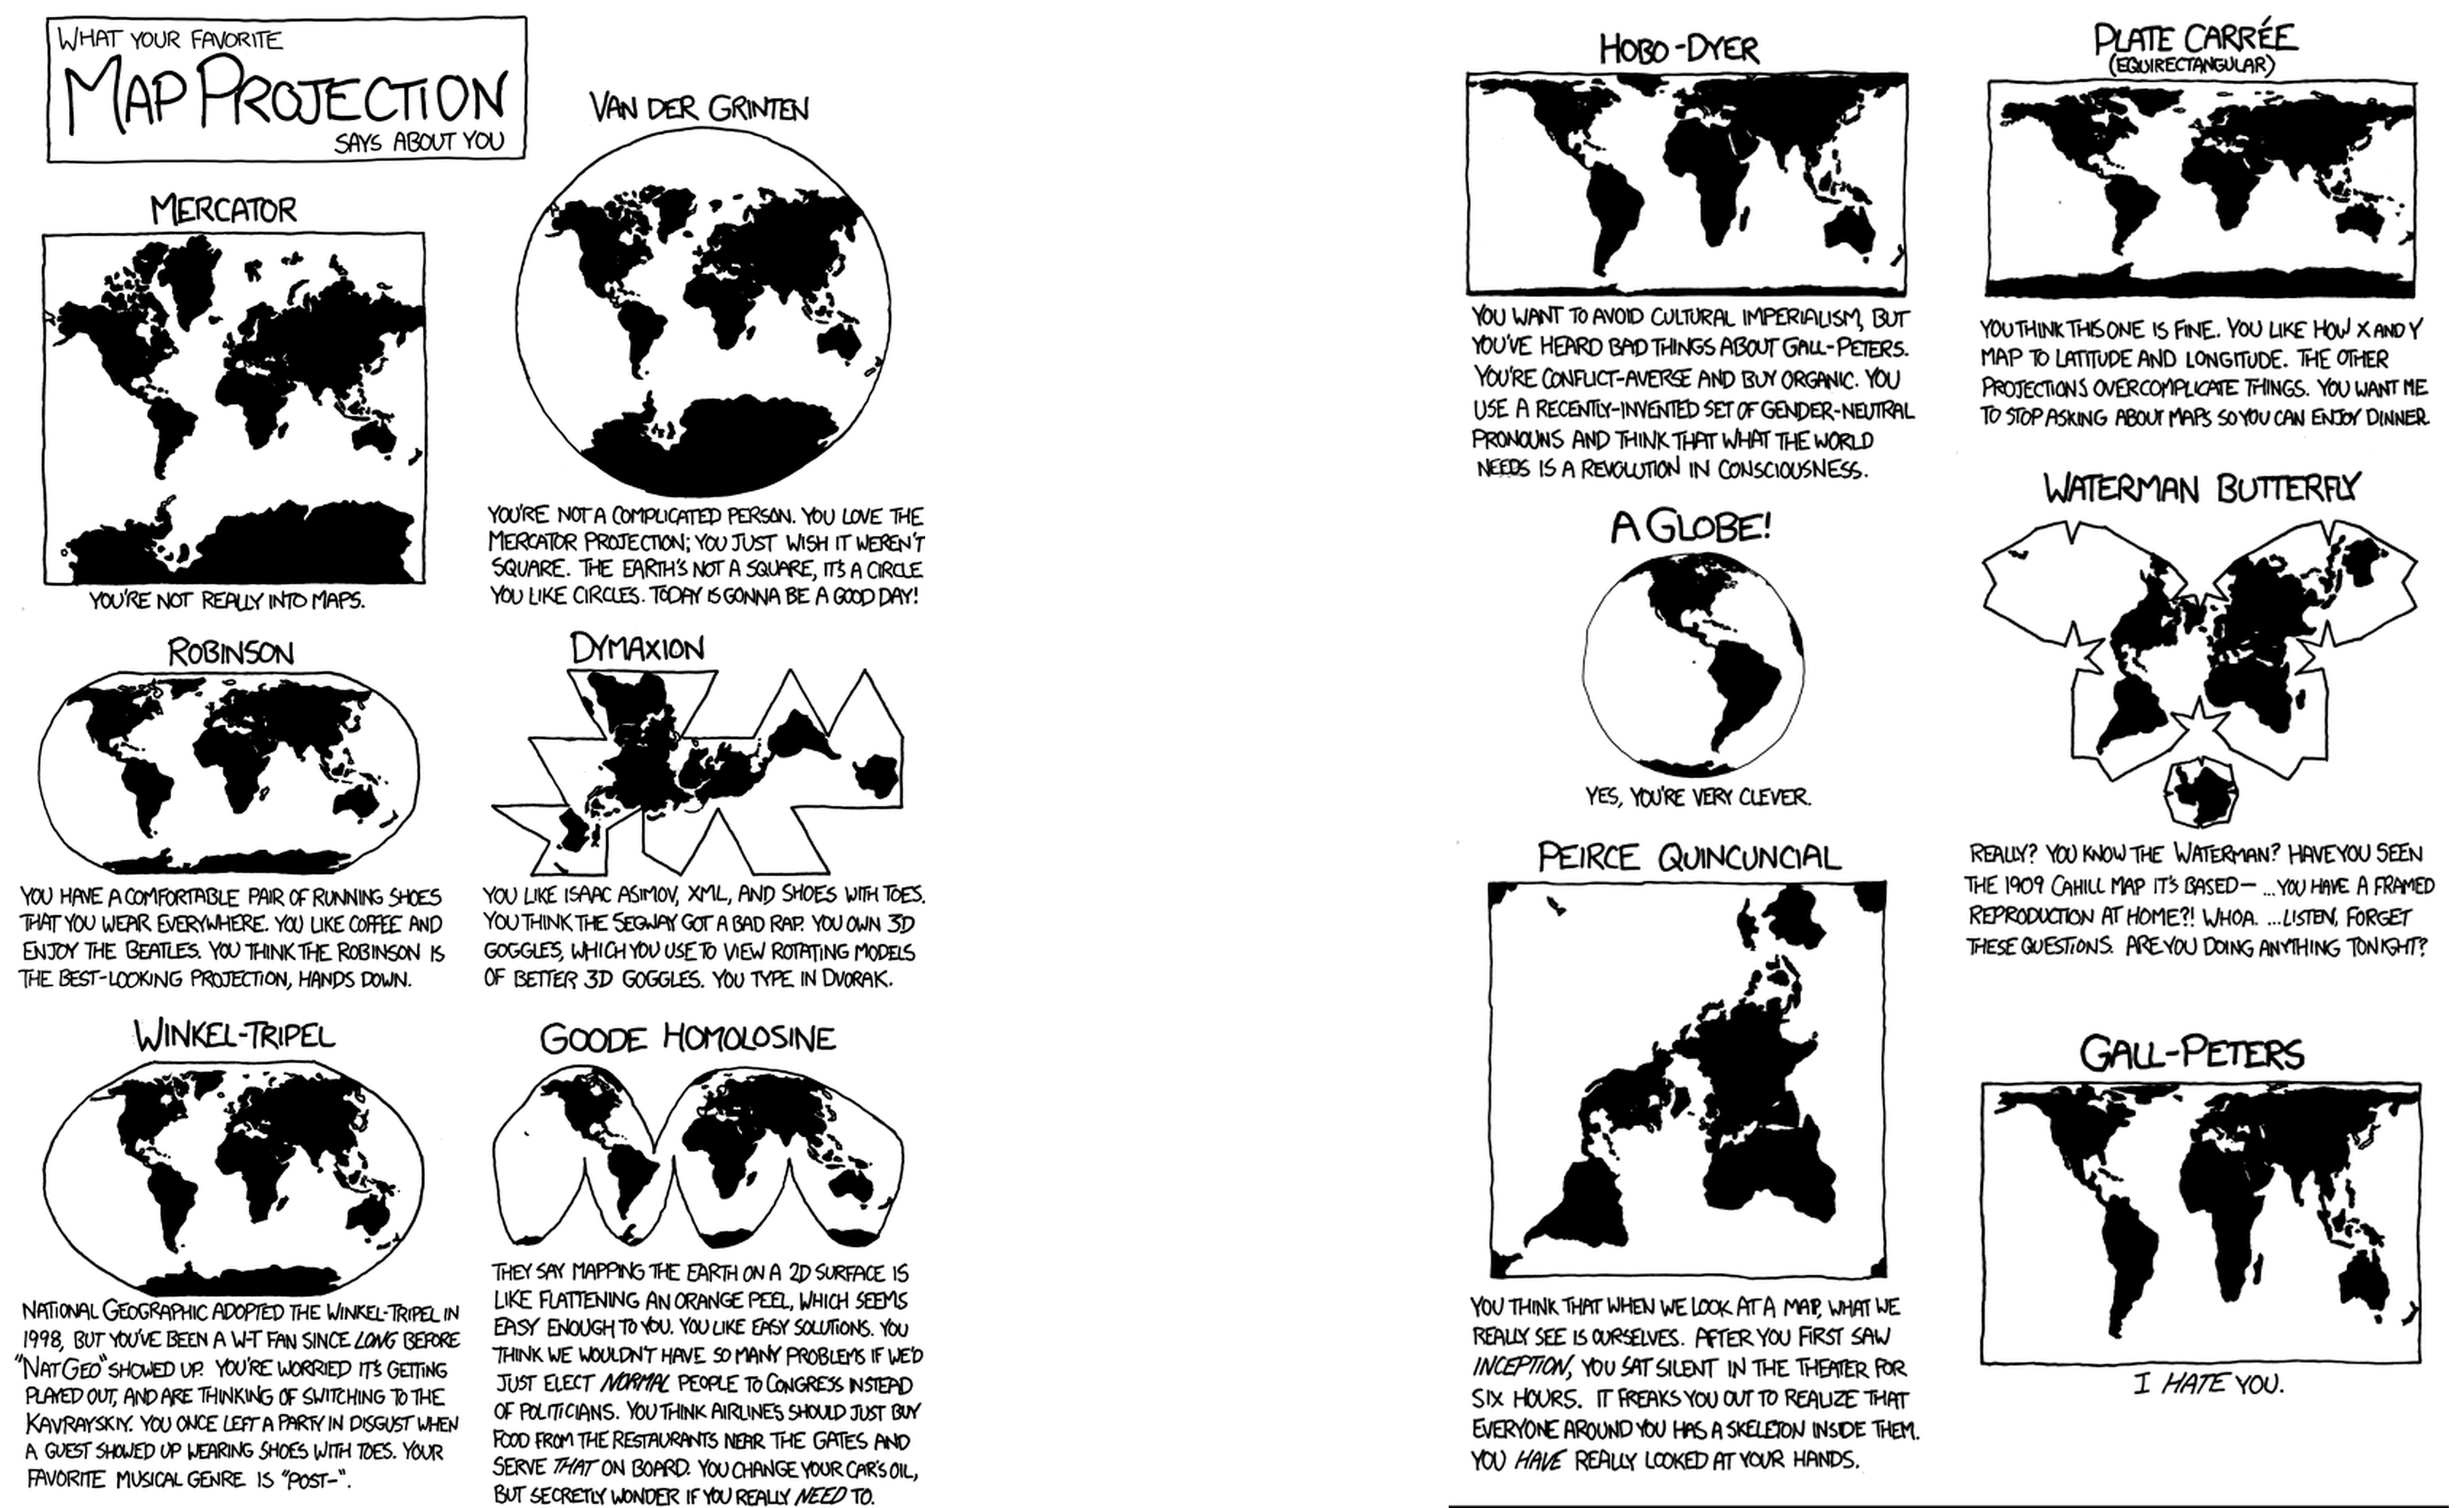
\includegraphics[width=\textwidth]{images/projections2}}%
}%

\caption{A quick introduction to projections\\ \ccbync~\href{http://xkcd.com/977/}{XKCD}}
\label{xkcd-projections}
\end{figure}

Before you go too deep into the world of projections you should download and (at least) skim \cite{snyder}. This will give you access to all the helpful maths that \GeoTools encodes for you (or if you are unlucky that you will need to add a new projection to the library).

\section{How to reproject features in \GeoTools}
\section{How to choose a ``good'' projection}